
%% bare_adv.tex
%% V1.4
%% 2012/12/27
%% by Michael Shell
%% See: 
%% http://www.michaelshell.org/
%% for current contact information.
%%
%% This is a skeleton file demonstrating the advanced use of IEEEtran.cls
%% (requires IEEEtran.cls version 1.8 or later) with an IEEE Computer
%% Society journal paper.
%%
%% Support sites:
%% http://www.michaelshell.org/tex/ieeetran/
%% http://www.ctan.org/tex-archive/macros/latex/contrib/IEEEtran/
%% and
%% http://www.ieee.org/

%%*************************************************************************
%% Legal Notice:
%% This code is offered as-is without any warranty either expressed or
%% implied; without even the implied warranty of MERCHANTABILITY or
%% FITNESS FOR A PARTICULAR PURPOSE! 
%% User assumes all risk.
%% In no event shall IEEE or any contributor to this code be liable for
%% any damages or losses, including, but not limited to, incidental,
%% consequential, or any other damages, resulting from the use or misuse
%% of any information contained here.
%%
%% All comments are the opinions of their respective authors and are not
%% necessarily endorsed by the IEEE.
%%
%% This work is distributed under the LaTeX Project Public License (LPPL)
%% ( http://www.latex-project.org/ ) version 1.3, and may be freely used,
%% distributed and modified. A copy of the LPPL, version 1.3, is included
%% in the base LaTeX documentation of all distributions of LaTeX released
%% 2003/12/01 or later.
%% Retain all contribution notices and credits.
%% ** Modified files should be clearly indicated as such, including  **
%% ** renaming them and changing author support contact information. **
%%
%% File list of work: IEEEtran.cls, IEEEtran_HOWTO.pdf, bare_adv.tex,
%%                    bare_conf.tex, bare_jrnl.tex, bare_jrnl_compsoc.tex,
%%                    bare_jrnl_transmag.tex
%%*************************************************************************

% *** Authors should verify (and, if needed, correct) their LaTeX system  ***
% *** with the testflow diagnostic prior to trusting their LaTeX platform ***
% *** with production work. IEEE's font choices can trigger bugs that do  ***
% *** not appear when using other class files.                            ***
% The testflow support page is at:
% http://www.michaelshell.org/tex/testflow/



% IEEEtran V1.7 and later provides for these CLASSINPUT macros to allow the
% user to reprogram some IEEEtran.cls defaults if needed. These settings
% override the internal defaults of IEEEtran.cls regardless of which class
% options are used. Do not use these unless you have good reason to do so as
% they can result in nonIEEE compliant documents. User beware. ;)
%
%\newcommand{\CLASSINPUTbaselinestretch}{1.0} % baselinestretch
%\newcommand{\CLASSINPUTinnersidemargin}{1in} % inner side margin
%\newcommand{\CLASSINPUToutersidemargin}{1in} % outer side margin
%\newcommand{\CLASSINPUTtoptextmargin}{1in}   % top text margin
%\newcommand{\CLASSINPUTbottomtextmargin}{1in}% bottom text margin



% Note that the a4paper option is mainly intended so that authors in
% countries using A4 can easily print to A4 and see how their papers will
% look in print - the typesetting of the document will not typically be
% affected with changes in paper size (but the bottom and side margins will).
% Use the testflow package mentioned above to verify correct handling of
% both paper sizes by the user's LaTeX system.
%
% Also note that the "draftcls" or "draftclsnofoot", not "draft", option
% should be used if it is desired that the figures are to be displayed in
% draft mode.
%
\newcommand{\irptitle}{Remaining Anonymous when using the Bitcoin digital currency}
\documentclass[10pt,conference]{IEEEtran}
% The Computer Society requires 12pt.
% If IEEEtran.cls has not been installed into the LaTeX system files,
% manually specify the path to it like:
% \documentclass[10pt,journal,compsoc]{../sty/IEEEtran}


% For Computer Society journals, IEEEtran defaults to the use of 
% Palatino/Palladio as is done in IEEE Computer Society journals.
% To go back to Times Roman, you can use this code:
%\renewcommand{\rmdefault}{ptm}\selectfont





% Some very useful LaTeX packages include:
% (uncomment the ones you want to load)



% *** MISC UTILITY PACKAGES ***
%
%\usepackage{ifpdf}
% Heiko Oberdiek's ifpdf.sty is very useful if you need conditional
% compilation based on whether the output is pdf or dvi.
% usage:
% \ifpdf
%   % pdf code
% \else
%   % dvi code
% \fi
% The latest version of ifpdf.sty can be obtained from:
% http://www.ctan.org/tex-archive/macros/latex/contrib/oberdiek/
% Also, note that IEEEtran.cls V1.7 and later provides a builtin
% \ifCLASSINFOpdf conditional that works the same way.
% When switching from latex to pdflatex and vice-versa, the compiler may
% have to be run twice to clear warning/error messages.






% *** CITATION PACKAGES ***
%
\ifCLASSOPTIONcompsoc
  % IEEE Computer Society needs nocompress option
  % requires cite.sty v4.0 or later (November 2003)
  % \usepackage[nocompress]{cite}
\else
  % normal IEEE
  % \usepackage{cite}
\fi
% cite.sty was written by Donald Arseneau
% V1.6 and later of IEEEtran pre-defines the format of the cite.sty package
% \cite{} output to follow that of IEEE. Loading the cite package will
% result in citation numbers being automatically sorted and properly
% "compressed/ranged". e.g., [1], [9], [2], [7], [5], [6] without using
% cite.sty will become [1], [2], [5]--[7], [9] using cite.sty. cite.sty's
% \cite will automatically add leading space, if needed. Use cite.sty's
% noadjust option (cite.sty V3.8 and later) if you want to turn this off
% such as if a citation ever needs to be enclosed in parenthesis.
% cite.sty is already installed on most LaTeX systems. Be sure and use
% version 4.0 (2003-05-27) and later if using hyperref.sty. cite.sty does
% not currently provide for hyperlinked citations.
% The latest version can be obtained at:
% http://www.ctan.org/tex-archive/macros/latex/contrib/cite/
% The documentation is contained in the cite.sty file itself.
%
% Note that some packages require special options to format as the Computer
% Society requires. In particular, Computer Society  papers do not use
% compressed citation ranges as is done in typical IEEE papers
% (e.g., [1]-[4]). Instead, they list every citation separately in order
% (e.g., [1], [2], [3], [4]). To get the latter we need to load the cite
% package with the nocompress option which is supported by cite.sty v4.0
% and later.
%
% Note also the use of a CLASSOPTION conditional provided by 
% IEEEtran.cls V1.7 and later.


\usepackage[style=ieee]{biblatex}
\addbibresource{i-d.bib}
\addbibresource{report.bib}
\addbibresource{rfc.bib}


% *** GRAPHICS RELATED PACKAGES ***
%
\ifCLASSINFOpdf
  \usepackage[pdftex]{graphicx}
  % declare the path(s) where your graphic files are
  % \graphicspath{{../pdf/}{../jpeg/}}
  % and their extensions so you won't have to specify these with
  % every instance of \includegraphics
  % \DeclareGraphicsExtensions{.pdf,.jpeg,.png}
\else
  % or other class option (dvipsone, dvipdf, if not using dvips). graphicx
  % will default to the driver specified in the system graphics.cfg if no
  % driver is specified.
  % \usepackage[dvips]{graphicx}
  % declare the path(s) where your graphic files are
  % \graphicspath{{../eps/}}
  % and their extensions so you won't have to specify these with
  % every instance of \includegraphics
  % \DeclareGraphicsExtensions{.eps}
\fi
% graphicx was written by David Carlisle and Sebastian Rahtz. It is
% required if you want graphics, photos, etc. graphicx.sty is already
% installed on most LaTeX systems. The latest version and documentation
% can be obtained at: 
% http://www.ctan.org/tex-archive/macros/latex/required/graphics/
% Another good source of documentation is "Using Imported Graphics in
% LaTeX2e" by Keith Reckdahl which can be found at:
% http://www.ctan.org/tex-archive/info/epslatex/
%
% latex, and pdflatex in dvi mode, support graphics in encapsulated
% postscript (.eps) format. pdflatex in pdf mode supports graphics
% in .pdf, .jpeg, .png and .mps (metapost) formats. Users should ensure
% that all non-photo figures use a vector format (.eps, .pdf, .mps) and
% not a bitmapped formats (.jpeg, .png). IEEE frowns on bitmapped formats
% which can result in "jaggedy"/blurry rendering of lines and letters as
% well as large increases in file sizes.
%
% You can find documentation about the pdfTeX application at:
% http://www.tug.org/applications/pdftex





% *** MATH PACKAGES ***
%
%\usepackage[cmex10]{amsmath}
% A popular package from the American Mathematical Society that provides
% many useful and powerful commands for dealing with mathematics. If using
% it, be sure to load this package with the cmex10 option to ensure that
% only type 1 fonts will utilized at all point sizes. Without this option,
% it is possible that some math symbols, particularly those within
% footnotes, will be rendered in bitmap form which will result in a
% document that can not be IEEE Xplore compliant!
%
% Also, note that the amsmath package sets \interdisplaylinepenalty to 10000
% thus preventing page breaks from occurring within multiline equations. Use:
%\interdisplaylinepenalty=2500
% after loading amsmath to restore such page breaks as IEEEtran.cls normally
% does. amsmath.sty is already installed on most LaTeX systems. The latest
% version and documentation can be obtained at:
% http://www.ctan.org/tex-archive/macros/latex/required/amslatex/math/





% *** SPECIALIZED LIST PACKAGES ***
%\usepackage{acronym}
% acronym.sty was written by Tobias Oetiker. This package provides tools for
% managing documents with large numbers of acronyms. (You don't *have* to
% use this package - unless you have a lot of acronyms, you may feel that
% such package management of them is bit of an overkill.)
% Do note that the acronym environment (which lists acronyms) will have a
% problem when used under IEEEtran.cls because acronym.sty relies on the
% description list environment - which IEEEtran.cls has customized for
% producing IEEE style lists. A workaround is to declared the longest
% label width via the IEEEtran.cls \IEEEiedlistdecl global control:
%
% \renewcommand{\IEEEiedlistdecl}{\IEEEsetlabelwidth{SONET}}
% \begin{acronym}
%
% \end{acronym}
% \renewcommand{\IEEEiedlistdecl}{\relax}% remember to reset \IEEEiedlistdecl
%
% instead of using the acronym environment's optional argument.
% The latest version and documentation can be obtained at:
% http://www.ctan.org/tex-archive/macros/latex/contrib/acronym/


%\usepackage{algorithmic}
% algorithmic.sty was written by Peter Williams and Rogerio Brito.
% This package provides an algorithmic environment fo describing algorithms.
% You can use the algorithmic environment in-text or within a figure
% environment to provide for a floating algorithm. Do NOT use the algorithm
% floating environment provided by algorithm.sty (by the same authors) or
% algorithm2e.sty (by Christophe Fiorio) as IEEE does not use dedicated
% algorithm float types and packages that provide these will not provide
% correct IEEE style captions. The latest version and documentation of
% algorithmic.sty can be obtained at:
% http://www.ctan.org/tex-archive/macros/latex/contrib/algorithms/
% There is also a support site at:
% http://algorithms.berlios.de/index.html
% Also of interest may be the (relatively newer and more customizable)
% algorithmicx.sty package by Szasz Janos:
% http://www.ctan.org/tex-archive/macros/latex/contrib/algorithmicx/




% *** ALIGNMENT PACKAGES ***
%
%\usepackage{array}
% Frank Mittelbach's and David Carlisle's array.sty patches and improves
% the standard LaTeX2e array and tabular environments to provide better
% appearance and additional user controls. As the default LaTeX2e table
% generation code is lacking to the point of almost being broken with
% respect to the quality of the end results, all users are strongly
% advised to use an enhanced (at the very least that provided by array.sty)
% set of table tools. array.sty is already installed on most systems. The
% latest version and documentation can be obtained at:
% http://www.ctan.org/tex-archive/macros/latex/required/tools/


%\usepackage{mdwmath}
%\usepackage{mdwtab}
% Also highly recommended is Mark Wooding's extremely powerful MDW tools,
% especially mdwmath.sty and mdwtab.sty which are used to format equations
% and tables, respectively. The MDWtools set is already installed on most
% LaTeX systems. The lastest version and documentation is available at:
% http://www.ctan.org/tex-archive/macros/latex/contrib/mdwtools/


% IEEEtran contains the IEEEeqnarray family of commands that can be used to
% generate multiline equations as well as matrices, tables, etc., of high
% quality.


%\usepackage{eqparbox}
% Also of notable interest is Scott Pakin's eqparbox package for creating
% (automatically sized) equal width boxes - aka "natural width parboxes".
% Available at:
% http://www.ctan.org/tex-archive/macros/latex/contrib/eqparbox/




% *** SUBFIGURE PACKAGES ***
%\ifCLASSOPTIONcompsoc
%  \usepackage[caption=false,font=normalsize,labelfont=sf,textfont=sf]{subfig}
%\else
%  \usepackage[caption=false,font=footnotesize]{subfig}
%\fi
% subfig.sty, written by Steven Douglas Cochran, is the modern replacement
% for subfigure.sty, the latter of which is no longer maintained and is
% incompatible with some LaTeX packages including fixltx2e. However,
% subfig.sty requires and automatically loads Axel Sommerfeldt's caption.sty
% which will override IEEEtran.cls' handling of captions and this will result
% in non-IEEE style figure/table captions. To prevent this problem, be sure
% and invoke subfig.sty's "caption=false" package option (available since
% subfig.sty version 1.3, 2005/06/28) as this is will preserve IEEEtran.cls
% handling of captions.
% Note that the Computer Society format requires a larger sans serif font
% than the serif footnote size font used in traditional IEEE formatting
% and thus the need to invoke different subfig.sty package options depending
% on whether compsoc mode has been enabled.
%
% The latest version and documentation of subfig.sty can be obtained at:
% http://www.ctan.org/tex-archive/macros/latex/contrib/subfig/




% *** FLOAT PACKAGES ***
%
%\usepackage{fixltx2e}
% fixltx2e, the successor to the earlier fix2col.sty, was written by
% Frank Mittelbach and David Carlisle. This package corrects a few problems
% in the LaTeX2e kernel, the most notable of which is that in current
% LaTeX2e releases, the ordering of single and double column floats is not
% guaranteed to be preserved. Thus, an unpatched LaTeX2e can allow a
% single column figure to be placed prior to an earlier double column
% figure. The latest version and documentation can be found at:
% http://www.ctan.org/tex-archive/macros/latex/base/


%\usepackage{stfloats}
% stfloats.sty was written by Sigitas Tolusis. This package gives LaTeX2e
% the ability to do double column floats at the bottom of the page as well
% as the top. (e.g., "\begin{figure*}[!b]" is not normally possible in
% LaTeX2e). It also provides a command:
%\fnbelowfloat
% to enable the placement of footnotes below bottom floats (the standard
% LaTeX2e kernel puts them above bottom floats). This is an invasive package
% which rewrites many portions of the LaTeX2e float routines. It may not work
% with other packages that modify the LaTeX2e float routines. The latest
% version and documentation can be obtained at:
% http://www.ctan.org/tex-archive/macros/latex/contrib/sttools/
% Do not use the stfloats baselinefloat ability as IEEE does not allow
% \baselineskip to stretch. Authors submitting work to the IEEE should note
% that IEEE rarely uses double column equations and that authors should try
% to avoid such use. Do not be tempted to use the cuted.sty or midfloat.sty
% packages (also by Sigitas Tolusis) as IEEE does not format its papers in
% such ways.
% Do not attempt to use stfloats with fixltx2e as they are incompatible.
% Instead, use Morten Hogholm'a dblfloatfix which combines the features
% of both fixltx2e and stfloats:
%
% \usepackage{dblfloatfix}
% The latest version can be found at:
% http://www.ctan.org/tex-archive/macros/latex/contrib/dblfloatfix/


%\ifCLASSOPTIONcaptionsoff
%  \usepackage[nomarkers]{endfloat}
% \let\MYoriglatexcaption\caption
% \renewcommand{\caption}[2][\relax]{\MYoriglatexcaption[#2]{#2}}
%\fi
% endfloat.sty was written by James Darrell McCauley, Jeff Goldberg and 
% Axel Sommerfeldt. This package may be useful when used in conjunction with 
% IEEEtran.cls'  captionsoff option. Some IEEE journals/societies require that
% submissions have lists of figures/tables at the end of the paper and that
% figures/tables without any captions are placed on a page by themselves at
% the end of the document. If needed, the draftcls IEEEtran class option or
% \CLASSINPUTbaselinestretch interface can be used to increase the line
% spacing as well. Be sure and use the nomarkers option of endfloat to
% prevent endfloat from "marking" where the figures would have been placed
% in the text. The two hack lines of code above are a slight modification of
% that suggested by in the endfloat docs (section 8.4.1) to ensure that
% the full captions always appear in the list of figures/tables - even if
% the user used the short optional argument of \caption[]{}.
% IEEE papers do not typically make use of \caption[]'s optional argument,
% so this should not be an issue. A similar trick can be used to disable
% captions of packages such as subfig.sty that lack options to turn off
% the subcaptions:
% For subfig.sty:
% \let\MYorigsubfloat\subfloat
% \renewcommand{\subfloat}[2][\relax]{\MYorigsubfloat[]{#2}}
% However, the above trick will not work if both optional arguments of
% the \subfloat command are used. Furthermore, there needs to be a
% description of each subfigure *somewhere* and endfloat does not add
% subfigure captions to its list of figures. Thus, the best approach is to
% avoid the use of subfigure captions (many IEEE journals avoid them anyway)
% and instead reference/explain all the subfigures within the main caption.
% The latest version of endfloat.sty and its documentation can obtained at:
% http://www.ctan.org/tex-archive/macros/latex/contrib/endfloat/
%
% The IEEEtran \ifCLASSOPTIONcaptionsoff conditional can also be used
% later in the document, say, to conditionally put the References on a 
% page by themselves.





% *** PDF, URL AND HYPERLINK PACKAGES ***
%
%\usepackage{url}
% url.sty was written by Donald Arseneau. It provides better support for
% handling and breaking URLs. url.sty is already installed on most LaTeX
% systems. The latest version and documentation can be obtained at:
% http://www.ctan.org/tex-archive/macros/latex/contrib/url/
% Basically, \url{my_url_here}.


% NOTE: PDF thumbnail features are not required in IEEE papers
%       and their use requires extra complexity and work.
%\ifCLASSINFOpdf
%  \usepackage[pdftex]{thumbpdf}
%\else
%  \usepackage[dvips]{thumbpdf}
%\fi
% thumbpdf.sty and its companion Perl utility were written by Heiko Oberdiek.
% It allows the user a way to produce PDF documents that contain fancy
% thumbnail images of each of the pages (which tools like acrobat reader can
% utilize). This is possible even when using dvi->ps->pdf workflow if the
% correct thumbpdf driver options are used. thumbpdf.sty incorporates the
% file containing the PDF thumbnail information (filename.tpm is used with
% dvips, filename.tpt is used with pdftex, where filename is the base name of
% your tex document) into the final ps or pdf output document. An external
% utility, the thumbpdf *Perl script* is needed to make these .tpm or .tpt
% thumbnail files from a .ps or .pdf version of the document (which obviously
% does not yet contain pdf thumbnails). Thus, one does a:
% 
% thumbpdf filename.pdf 
%
% to make a filename.tpt, and:
%
% thumbpdf --mode dvips filename.ps
%
% to make a filename.tpm which will then be loaded into the document by
% thumbpdf.sty the NEXT time the document is compiled (by pdflatex or
% latex->dvips->ps2pdf). Users must be careful to regenerate the .tpt and/or
% .tpm files if the main document changes and then to recompile the
% document to incorporate the revised thumbnails to ensure that thumbnails
% match the actual pages. It is easy to forget to do this!
% 
% Unix systems come with a Perl interpreter. However, MS Windows users
% will usually have to install a Perl interpreter so that the thumbpdf
% script can be run. The Ghostscript PS/PDF interpreter is also required.
% See the thumbpdf docs for details. The latest version and documentation
% can be obtained at.
% http://www.ctan.org/tex-archive/support/thumbpdf/


% NOTE: PDF hyperlink and bookmark features are not required in IEEE
%       papers and their use requires extra complexity and work.
% *** IF USING HYPERREF BE SURE AND CHANGE THE EXAMPLE PDF ***
% *** TITLE/SUBJECT/AUTHOR/KEYWORDS INFO BELOW!!           ***
\newcommand\MYhyperrefoptions{bookmarks=true,bookmarksnumbered=true,
pdfpagemode={UseOutlines},plainpages=false,pdfpagelabels=true,
colorlinks=true,linkcolor={black},citecolor={black},urlcolor={black},
pdftitle={\irptitle},%<!CHANGE!
pdfsubject={Bitcoin},%<!CHANGE!
pdfauthor={Thomas A. Grainger},%<!CHANGE!
pdfkeywords={Bitcoin, Anonymity, Cryptography, crypto-currencies, Peer to Peer}}%<^!CHANGE!
\ifCLASSINFOpdf
\usepackage[\MYhyperrefoptions,pdftex]{hyperref}
\else
\usepackage[\MYhyperrefoptions,breaklinks=true,dvips]{hyperref}
\usepackage{breakurl}
\fi
% One significant drawback of using hyperref under DVI output is that the
% LaTeX compiler cannot break URLs across lines or pages as can be done
% under pdfLaTeX's PDF output via the hyperref pdftex driver. This is
% probably the single most important capability distinction between the
% DVI and PDF output. Perhaps surprisingly, all the other PDF features
% (PDF bookmarks, thumbnails, etc.) can be preserved in
% .tex->.dvi->.ps->.pdf workflow if the respective packages/scripts are
% loaded/invoked with the correct driver options (dvips, etc.). 
% As most IEEE papers use URLs sparingly (mainly in the references), this
% may not be as big an issue as with other publications.
%
% That said, Vilar Camara Neto created his breakurl.sty package which
% permits hyperref to easily break URLs even in dvi mode.
% Note that breakurl, unlike most other packages, must be loaded
% AFTER hyperref. The latest version of breakurl and its documentation can
% be obtained at:
% http://www.ctan.org/tex-archive/macros/latex/contrib/breakurl/
% breakurl.sty is not for use under pdflatex pdf mode.
%
% The advanced features offer by hyperref.sty are not required for IEEE
% submission, so users should weigh these features against the added
% complexity of use.
% The package options above demonstrate how to enable PDF bookmarks
% (a type of table of contents viewable in Acrobat Reader) as well as
% PDF document information (title, subject, author and keywords) that is
% viewable in Acrobat reader's Document_Properties menu. PDF document
% information is also used extensively to automate the cataloging of PDF
% documents. The above set of options ensures that hyperlinks will not be
% colored in the text and thus will not be visible in the printed page,
% but will be active on "mouse over". USING COLORS OR OTHER HIGHLIGHTING
% OF HYPERLINKS CAN RESULT IN DOCUMENT REJECTION BY THE IEEE, especially if
% these appear on the "printed" page. IF IN DOUBT, ASK THE RELEVANT
% SUBMISSION EDITOR. You may need to add the option hypertexnames=false if
% you used duplicate equation numbers, etc., but this should not be needed
% in normal IEEE work.
% The latest version of hyperref and its documentation can be obtained at:
% http://www.ctan.org/tex-archive/macros/latex/contrib/hyperref/





% *** Do not adjust lengths that control margins, column widths, etc. ***
% *** Do not use packages that alter fonts (such as pslatex).         ***
% There should be no need to do such things with IEEEtran.cls V1.6 and later.
% (Unless specifically asked to do so by the journal or conference you plan
% to submit to, of course. )


% correct bad hyphenation here
\hyphenation{op-tical net-works semi-conduc-tor}
\usepackage{amssymb}
\usepackage{amsmath}

\begin{document}
%
% paper title
% can use linebreaks \\ within to get better formatting as desired
% Do not put math or special symbols in the title.
\title{\irptitle}
%
%
% author names and IEEE memberships
% note positions of commas and nonbreaking spaces ( ~ ) LaTeX will not break
% a structure at a ~ so this keeps an author's name from being broken across
% two lines.
% use \thanks{} to gain access to the first footnote area
% a separate \thanks must be used for each paragraph as LaTeX2e's \thanks
% was not built to handle multiple paragraphs
%
%
%\IEEEcompsocitemizethanks is a special \thanks that produces the bulleted
% lists the Computer Society journals use for "first footnote" author
% affiliations. Use \IEEEcompsocthanksitem which works much like \item
% for each affiliation group. When not in compsoc mode,
% \IEEEcompsocitemizethanks becomes like \thanks and
% \IEEEcompsocthanksitem becomes a line break with idention. This
% facilitates dual compilation, although admittedly the differences in the
% desired content of \author between the different types of papers makes a
% one-size-fits-all approach a daunting prospect. For instance, compsoc 
% journal papers have the author affiliations above the "Manuscript
% received ..."  text while in non-compsoc journals this is reversed. Sigh.

\author{\href{http://graingert.co.uk/foaf.rdf\#me}{Thomas~A.~Grainger}\protect\\
Electronics and Computer Science\protect\\
University of Southampton\protect\\
% note need leading \protect in front of \\ to get a newline within \thanks as
% \\ is fragile and will error, could use \hfil\break instead.
\href{mailto:t.grainger@ecs.soton.ac.uk}{Email:~t.grainger@ecs.soton.ac.uk}
}% <-this % stops a space

% note the % following the last \IEEEmembership and also \thanks - 
% these prevent an unwanted space from occurring between the last author name
% and the end of the author line. i.e., if you had this:
% 
% \author{....lastname \thanks{...} \thanks{...} }
%                     ^------------^------------^----Do not want these spaces!
%
% a space would be appended to the last name and could cause every name on that
% line to be shifted left slightly. This is one of those "LaTeX things". For
% instance, "\textbf{A} \textbf{B}" will typeset as "A B" not "AB". To get
% "AB" then you have to do: "\textbf{A}\textbf{B}"
% \thanks is no different in this regard, so shield the last } of each \thanks
% that ends a line with a % and do not let a space in before the next \thanks.
% Spaces after \IEEEmembership other than the last one are OK (and needed) as
% you are supposed to have spaces between the names. For what it is worth,
% this is a minor point as most people would not even notice if the said evil
% space somehow managed to creep in.



% The paper headers
%\markboth{Journal of \LaTeX\ Class Files,~Vol.~11, No.~4, December~2012}%
%{Shell \MakeLowercase{\textit{et al.}}: Bare Advanced Demo of IEEEtran.cls for Journals}
% The only time the second header will appear is for the odd numbered pages
% after the title page when using the twoside option.
% 
% *** Note that you probably will NOT want to include the author's ***
% *** name in the headers of peer review papers.                   ***
% You can use \ifCLASSOPTIONpeerreview for conditional compilation here if
% you desire.



% The publisher's ID mark at the bottom of the page is less important with
% Computer Society journal papers as those publications place the marks
% outside of the main text columns and, therefore, unlike regular IEEE
% journals, the available text space is not reduced by their presence.
% If you want to put a publisher's ID mark on the page you can do it like
% this:
%\IEEEpubid{0000--0000/00\$00.00~\copyright~2012 IEEE}
% or like this to get the Computer Society new two part style.
%\IEEEpubid{\makebox[\columnwidth]{\hfill 0000--0000/00/\$00.00~\copyright~2012 IEEE}%
%\hspace{\columnsep}\makebox[\columnwidth]{Published by the IEEE Computer Society\hfill}}
% Remember, if you use this you must call \IEEEpubidadjcol in the second
% column for its text to clear the IEEEpubid mark (Computer Society journal
% papers don't need this extra clearance.)



% use for special paper notices
%\IEEEspecialpapernotice{(Invited Paper)}




% for Computer Society papers, we must declare the abstract and index terms
% PRIOR to the title within the \IEEEtitleabstractindextext IEEEtran
% command as these need to go into the title area created by \maketitle.
% As a general rule, do not put math, special symbols or citations
% in the abstract or keywords.
\IEEEtitleabstractindextext{%

\begin{abstract}
The abstract goes here.
\end{abstract}
}


% make the title area
\maketitle


% To allow for easy dual compilation without having to reenter the
% abstract/keywords data, the \IEEEtitleabstractindextext text will
% not be used in maketitle, but will appear (i.e., to be "transported")
% here as \IEEEdisplaynontitleabstractindextext when compsoc mode
% is not selected <OR> if conference mode is selected - because compsoc
% conference papers position the abstract like regular (non-compsoc)
% papers do!
\IEEEdisplaynontitleabstractindextext
% \IEEEdisplaynontitleabstractindextext has no effect when using
% compsoc under a non-conference mode.


% For peer review papers, you can put extra information on the cover
% page as needed:
% \ifCLASSOPTIONpeerreview
% \begin{center} \bfseries EDICS Category: 3-BBND \end{center}
% \fi
%
% For peerreview papers, this IEEEtran command inserts a page break and
% creates the second title. It will be ignored for other modes.
\IEEEpeerreviewmaketitle

%Remaining Anonymous when using the Bitcoin Protocol
\section{Introduction}
% Computer Society journal papers do something a tad strange with the very first
% section heading (almost always called "Introduction"). They place it ABOVE the
% main text! IEEEtran.cls currently does not do this for you.  However, You can
% achieve this effect by making LaTeX jump through some hoops via something
% like:
%
%\ifCLASSOPTIONcompsoc \noindent\raisebox{2\baselineskip}[0pt][0pt]%
%{\parbox{\columnwidth}{\section{Introduction}\label{sec:introduction}%
%\global\everypar=\everypar}}% \vspace{-1\baselineskip}\vspace{-\parskip}\par
%\else \section{Introduction}\label{sec:introduction}\par \fi
%
% Admittedly, this is a hack and may well be fragile, but seems to do the trick
% for me. Note the need to keep any \label that may be used right after \section
% in the above as the hack puts \section within a raised box.



% The very first letter is a 2 line initial drop letter followed by the rest of
% the first word in caps (small caps for compsoc).
% 
% form to use if the first word consists of a single letter:
% \IEEEPARstart{A}{demo} file is ....
% 
% form to use if you need the single drop letter followed by normal text
% (unknown if ever used by IEEE): \IEEEPARstart{A}{}demo file is ....
% 
% Some journals put the first two words in caps: \IEEEPARstart{T}{his demo} file
% is ....
% 
% Here we have the typical use of a "T" for an initial drop letter and "HIS" in
% caps to complete the first word.
%\IEEEPARstart{T}{his}

At 6:15 pm on the 3rd of January 2009, Satoshi Nakamoto (likely a pseudonym) created and announced a block of data known as the `Genesis Block' of the Bitcoin block chain~\cite{satoshi}. With this block, the first 50 units of the decentralized peer to peer currency, Bitcoin, were created\footnote{Strictly this isn't true, as due to a bug in the bitcoin client the first 50 bitcoins created cannot actually be spent.}. Since then, over ten million bitcoins have been generated.

The \textcite{euro-currency-schemes} (ECB) describes three different virtual currency schemes: closed currency schemes, unidirectional and bidirectional flow currency schemes.  Closed currency schemes involve currencies that cannot be converted to or from fiat currency\footnote{Fiat currency is a currency with a value given by government regulation such as the Great British Pound (GBP) or the United States Dollar (USD)}, an example of this would be `World of Warcraft gold'\footnote{\url{http://eu.battle.net/wow/en/shop/anti-gold/}} which cannot be bought using legal tender without violating the terms of service.  Unidirectional currency schemes include currencies like `Facebook Credits'\footnote{\url{https://www.facebook.com/credits/}} that can be purchased using legal tender but cannot be transfered to other users.  Finally, bidirectional currency schemes describe currency which can be converted to and from fiat currency, bitcoins are an example of this and are currently trading at \input{price}.

Bitcoin is distinct from other bidirectional digital currency schemes such as central banking and financial institutions or money transfer systems such as PayPal\cite{paypal} in that ``it is neither created nor administered by a single authority such as a central bank''\cite{why-interesting}, transactions are also irreversible are made pseudo-anonymously. The bitcoin protocol allows multiple different clients to connect, verify and disseminate transactions.  The reference bitcoin client, has received multiple releases\footnote{\url{http://bitcoin.org/en/version-history\#0.5.0}} and is now known as Bitcoin-Qt\cite{bitcoin-qt}. For the sake of brevity this paper will refer to Bitcoin-Qt Bitcoin client as the Bitcoin client.

\section{Related Work}
Research on the Bitcoin protocol has mostly centered around proposing improvements to the protocol, such as the \textcite{red-balloons} who sugggest a reward scheme for ensuring bitcoin peers tranfer transactions, or \textcite{bitter-to-better} that looks at a multitude of different proposals for improvement.  Other research such as that of \textcite{legal}, focus on the legal status of bitcoin as a currency.  This research paper focusses on the emergance, from other digital currencies, and the anonymity of the Bitcoin protocol.

\section{Background}
The core of any currency is to allow users to participate in transactions that result in transfer of value between the participants.  Such a system requires an element of trust or protocols that remove the need for trust between the participants.  If a user, Alice, wishes to send some value to Bob, Bob will need to know that Alice has the funds to send that transaction and has not sent or allocated that money to anyone else (a double spend). This problem is easily solvable using a physical transferable goods where the expense to duplicate or create more of a resource can be ensured to be more than the value of the item: for example creating counterfeit paper currency or creating a commodity like gold.  Although the issue of trust is somewhat negated with physical goods, they also encounter a separate issue - moving that value over distance.  This can be an expensive exercise as it requires both the expense of physically moving the good - particularly an issue with heavy gold bars - as well as the cost of securing it during transportation. While paper currencies solve these problems somewhat, with a trade-off of making duplication easier, a digital currency aims to recreate the difficulty in duplication, while taking advantage of the ease of transfer that digital information brings.

Up until relatively recently, discussions in scientific literature surrounding currency systems have assumed the necessity of some type of trusted central authority or authorities as part of the operation of the protocol.  These authorities usually maintain a record of transactions performed as well as minting and controlling the currency.  However, the relative success of Bitcoin has shown that this assumption is not necessarily the case and has increased discussion into decentralised currency - moving it from a topic of intellectual curiosity to one with more practical implications.

\subsection{Central Banking Authorities}

===================================================
===================================================
Services such as the UK ``Faster Payments Service''~\cite{guardian-fps}, or the ``Single Euro Payments Area'' (SEPA) payments initiative~\cite{SEPA} operate as a transfer protocol between users of trusted entities such as banks and other financial institutions.  While, payment processor systems and services, such as PayPal\footnote{\url{https://www.paypal.com/uk/webapps/mpp/transfer-money-online}}, Dwolla\footnote{\url{https://www.dwolla.com/individuals}} and Liberty Reserve\footnote{\url{http://web.archive.org/web/20130430103158/http://www.libertyreserve.com/}} operate on-top of existing currencies and, in exchange for money sent using SEPA or bank transfer, allow accounts to be credited with the equivalent value.  When a user requests a value transfer one account is debited while another is credited~\cite{paypal}.

While there are legal distinction between financial institutions and payment processors there is no significant technical distinction. These systems are effectively fully centralized, digital systems of exchange in which only the central authority or authorities control the minting of the currency or are able to create transactions.  An individual cannot create transactions and must rely on the central authority to make the transaction on their behalf.

These fully centralized systems have a simple design and implementation and often provide useful features such as insurance and interest.  However, during the operation of these systems some key disadvantages for the users have become apparent: the trusted entities have a legal responsibility to handle ``charge-backs'' or reverse transactions, the cost for this escrow service is placed on the customer as a transfer fee or to the merchant as a fine in the case of escrow failure. The second major disadvantage of these systems is that they are liable to be closed down due to legal pressure~\cite{lr-shutdown,lr-idictment}, or individual users' accounts can be frozen~\cite{mtgox-dwolla,vlad:mtgox-dwolla}.

In  systems where some trusted central authority exists, while it may be  reasonable to trust  some agent for the purpose of authenticating the  ownership of  value, that authority may act in a way outside of the  agents' control.  For example, if the server hosting the system is  compromised either through technical or legal means.

%uh oh this is duplicated...?
These fully centralized systems have a simple design and implementation however, there are some key issues that affect the users of the system - both merchants and customers - two of which are discussed here.  

The first issue is that the trusted entity has a legal responsibility to handle ``charge-backs'' or reverse transactions, the cost for this escrow service - in which the central authority acts as an arbiter in disputes - is placed on the customer as a transfer fee or to the merchant as a fine, or worse\cite{violin}.

The second major disadvantage of a centralized system is that it allows for  a single point of failure resulting in a lack of reliability from the  perspective of the user.  The central authority has complete control over the status of the users' account - that authority can freeze the funds of that account at their discretion according to their own terms of service, this can include pressure from legal authorities~\cite{mtgox-dwolla,vlad:mtgox-dwolla,wikileaks-paypal}.  Additionally, the central authority exists as an easier target for legal action, should that authority fail to freeze or track `problematic' accounts and this may result in a total shut down of that service~\cite{lr-shutdown,egold-shutdown,lr-idictment}. This report assumes that being resistant to attack from a third party, regardless of the good intentions of that party, is an advantageous feature of a currency.  It is not in the scope of this report to discuss the legal or ethical repercussions of such a system.

=============================================================

\subsection{Unique Token}
\textcite{netcash} discuss one solution, NetCash.  This protocol uses a unique token held by both the central authority and the owner of the coin. To create NetCash currency, the user and central authority agree on a unique token in exchange for some currency or resource. When that user wishes to transact value to another, they simply send the token to the other user.  A receiver can opt to trust the sender, thus remaining anonymous, or can trade-off anonymity for an assurance of validity from the central server.  To verify that the transaction is legitimate, receiving users send the token to the exchange, to be swapped for a new spendable token meaning the original token can no longer be spent. One issue with this protocol is the central authority cannot be independently verified, as such the central server may deny knowledge of a valid token, or allow multiple users to claim the same token and arbitrarily mint new tokens without a fee (either maliciously, due to being compromised or due to data loss).

\subsection{Blind-signed Chaumian e-Cash}
Proposed by \textcite{chaum}, the Chaum Token protocol, uses blind signatures. A user, Alice, creates a token $x$ and blinds it using function $c$.  A central authority will sign this blinded message using signing function $s$ in exchange for a fee, creating $s(c(x)$.  The authority then returns the blind signed message to Alice. Alice then removes the blind, leaving the signature $s(x)$ using $c^{-1}(s(c(x)))$.  These signed messages can now operate in a similar manner to tokens from the NetCash system: Alice can send $s(x)$ to Bob, who verifies the central authority's signature, and is now able to redeem this token with the central authority preventing Alice from sending the same token to another user.

The blinding protocol has the advantage that the central authority cannot discover the previous owner of a signed message when cashed by a payee because it is assumed that $c(x)$ cannot be derived from $s(x)$.  This protocol, however, maintains similar issues to NetCash: the central server may allow multiple users to claim the same token and arbitrarily mint new tokens without a fee (either maliciously, due to being compromised or due to data loss).

In both NetCash and Chaumian e-Cash the central server may accuse the original owner of the token of double spending the transaction.  Assuming Alice did not double spend the token, she now knows that the central server is dishonest, Bob on the other-hand cannot determine which of Alice or the central authority are being dishonest.

\subsection{B-Money digital signature chain}\label{digital-sig}
An alternative solution, B-Money proposed by~\textcite{b-money}, uses a chain of digital signatures where transaction messages are created using public key cryptography and the chain of digital signatures can be traced back to the original creation of the unit of value. In this system money is not sent per-se (only the transaction messages themselves are sent) but re-assigned.

``If Alice (owner of pseudonym $K_A$) wishes to transfer X units of money to Bob (owner of pseudonym $K_B$), she broadcasts the message ``I give X units of money to $K_B$'' signed by $K_A$'' for example see Figure~\ref{fig:chain-spend}.

This system presents the same problems as before regarding value distribution and potential double spending i.e. how does Bob know that Alice has the value to start with and how does Bob know that this value hasn't already been spent.  Figure~\ref{fig:chain-double-spend} gives an example of how a double spend might occur. \textcite{b-money} proposes two solutions to this problem: using a theoretical but impossible ``synchronous and unjammable anonymous broadcast channel'' or alternatively, to involve multiple trusted authorities that host a public copy of every transaction sent - if these peers attempt to show a differing view of history then fines can be levied from another peer.

Bob can download a copy of the transaction chain from one of these servers and verify that Alice was given some value from a chain of transactions leading back to the central authority where the value is assumed to be created and can subtract the total value of  Alice's spent transactions to determine if the transaction sent to Bob is valid.

\begin{figure}[t!]
    \centering
    
\includegraphics[width=\columnwidth]{img/Bitcoin_Transaction_Visual}
    \caption{A chain of digital signatures representing value transfer.
    (source \protect\cite{satoshi})}
    \label{fig:chain-spend}
\end{figure}

\begin{figure}[t!]
    \centering
    
\includegraphics[width=\columnwidth]{img/Bitcoin_DoubleSpend_Visual}
    \caption{A chain of digital signatures representing value transfer with a double spend: Without some consensus system ``User 2'' is not prevented from sending the same value to both ``Owner 3'' and ``Owner 4''.
    (based on work from \protect\cite{satoshi})}
    \label{fig:chain-double-spend}
\end{figure}

The central authorities in this protocol also requires some degree of trust from the user that the authority is both benign and secure. For example, the central authorities could cooperate with, or more simply act as, a user attempting to achieve a double spend attack by showing different views to different users. Another reason that this currency was not adopted, was that a concrete implementation was never created and servers were never elected.

\section{The Bitcoin Protocol}
The Bitcoin protocol and client software~\textcite{satoshi} makes very few changes to the original b-money\cite{b-money} proposal. 

The Bitcoin protocol and client software provides a concrete implementation of an altered version of the original b-money proposal, with defined transaction syntax such as dynamic payment scripts and the concept of outputs that must be spent in their entirety.  The only significant novel deviation is that \textcite{satoshi} has substituted the ``synchronous and unjammable anonymous broadcast channel''~\cite{b-money} with a decentralized time stamp server that is used to ratify the order in which transactions occurred.  This allows for a dynamically changing set of transaction authorizing servers to achieve a consensus of valid transactions. Any user can, on receipt of a transaction, query the time stamp server and determine whether a transaction has been invalidated by a prior transaction. This key difference is likely the reason that Bitcoin took crypto-currencies from mathematical curiosity to a usable system for storage and transfer of value.

\subsection{Distributed Transaction Validation}
During the operation of the distributed time stamp server, the Bitcoin peer network, creates a chain of blocks of transactions, each referring to the previous by hash value. This is known as the Bitcoin block chain.  The transactions to be included in blocks in the chain are discovered when peers broadcast them into a peer discovery network that operates in a similar manner to a BitTorrent swarm\cite{swarm}.  Any user can contribute to this chain of blocks, but before another peer will relay it to others, it must meet a ``proof-of-work'' requirement: the double SHA-256 hash value of each block must not exceed a value determined by the current `difficulty'.  Because the SHA2 hashing function has been designed such that the value of an amount of data is unpredictable and evenly distributed in the range of the function, the only way for a participant to create data with a hash value below the difficulty limit is to repeatedly try different input data values\cite{btc-crypto}.  \textcite{satoshi} stated that ``The average work required is exponential in the number of zero bits required and can be verified by executing a single hash''. Transaction block data can be altered without changing the transaction semantics because the block format includes a `nonce' field for this purpose.

Because each block refers to the previous block, ``To modify a past block, an attacker would have to redo the proof-of-work of the block and all blocks after it''.  A peer in the Bitcoin network will accept a block if it has the highest total difficulty of any other block at that block height, shown in figure~\ref{ref:blockchain}, this allows the block chain to temporarily fork in the case that two blocks are created at the same time. The required difficulty of a valid block is re-calculated every 2016 blocks to ensure that block production takes the entire network an average of 10 minutes to solve.

\begin{figure}[t!]
    \centering
    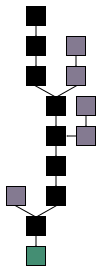
\includegraphics[height=\columnwidth]{img/Blockchain}
    \caption{A diagram showing invalid blocks (grey) being invalidated by a block chain with greater totaly difficulty (black). (based on work from theymos\protect\footnote{\url{http://theymos.com/}})}
    \label{fig:blockchain}
\end{figure}

As more blocks are created the more expensive it is for any group to alter the consensus reached by the peer network.  Because the proof of work system is computationally expensive, an incentive (other than the increased certainty of any transaction a user has previously received will remain valid) is included.  

While it is required that transactions included in a block have a total input value that exceeds the output value, one transaction, the `coinbase' transaction, can be included with no input and has a reward output.  The reward output is limited to the total difference between the input and output values of all other transactions in the block (as transaction fees), and a number related to the total number of blocks created by the network. Currently this reward is 25 bitcoins plus fees and is specified to halve every four years worth of blocks.  The intention is that the creator of the block assigns that reward to their own public key or address. This reward is `paid' for by the consensual deflation of every participants' held bitcoin. This process also serves to solve the distribution problem of digital currencies.

\subsection{The Bitcoin block-chain is not strictly a consensus protocol}
\textcite{bitcoin-impossible} notes that, strictly, the Bitcoin proof of work block chain is not a consensus scheme. In distributed consensus protocols, consensus is arrived at when some sufficient number of members of the group agree.

This is impossible to achieve in a distributed system where this group is not known (agents are constantly joining and leaving the group) in a way that prevents Sybil attacks\cite{sybil} where an individual represents themselves as many agents, with the aim of overriding the group consensus.  By declaring the Bitcoin group consensus definition as ``all the computing power in existence'' consensus is only achieved once more than half of the compute power in existence is used in the proof of work system. Therefore the Bitcoin system is only Sybil \emph{resistant}. The Bitcoin systems is also not fully decentralized, a set of core developers, now the Bitcoin Foundation, have some control over the protocol; two major disruptions to the network have been solved using manual intervention from this group.  The first occurred on 15 August 2010 when an integer overflow was discovered in the Bitcoin protocol, this vulnerability ``allows remote attackers to bypass intended economic restrictions and create many bitcoins via a crafted Bitcoin transaction.''~\cite{CVE-2010-5139}. The second was when the network segmented two groups of clients with two differing consensus conclusions~\cite{CVE-2013-3220,glitch-report,major-glitch}.  Users of the network are still free to ignore the advice of this group by opting not to update or alter their clients in doing so permanently segregating themselves from the rest of the network.

\section{Anonymity}
As part of the Bitcoin protocol, all transactions must be broadcast publicly.  However, \textcite{satoshi} maintains that ``privacy can still be maintained by breaking the flow of information [...] by keeping public keys anonymous''.

Each Bitcoin address can be considered a pseudonym of the owner of it's associated private key, and because each person can own multiple Bitcoin addresses in a wallet there is a disconnect between users and addresses. \textcite{satoshi} asserts that because of this disconnect between users and addresses it is difficult to associate a particular transaction with a particular user.

\subsection{Taint Analysis}
\textcite{reid-anon}, consider the feasibility of maintaining this pseudo-anonymity in practise, by investigating the multiple input semantics of the Bitcoin transaction format. They argue that any key taking part in this process was in a single wallet, and thus owned by a single user. Therefore by combining the knowledge of how keys are grouped into wallets with knowledge from outside the protocol other inferences can be made, with the aim to determine the identity of the user behind the wallet, and thus any transactions made.  The proposed method for de-anonymizing a user occurs in two phases.  First, the publicly available ``transaction network'', as published in the block chain, is contracted to a ``user network'' by determining groups of addresses that appear to behave as part of a single wallet.  The second phase is to link that group with an identity using publicly available ``Off-Network Information'' linking users to any address in that group, e.g. by crawling the web for forum posts including both user-names and addresses.  \textcite{eval-priv} add to this a further heuristic of ``Shadow Addresses'' to associate newly created addresses with users.

\subsubsection{Multi-input Transactions}
In the Bitcoin transaction format, if a user cannot fulfil the value of a transaction by spending a single previous output, the client will combine multiple inputs, where the user has the ability to fulfil their spend conditions.  When combined, the Bitcoin client must fulfil the spend conditions of all of the inputs, usually the conditions result in the requirement to sign the transaction with all of the participating address's private keys.  ``It is therefore straightforward to conclude that if these (inputs) are (spendable) by different addresses, then the input addresses belong to the same user''\cite{eval-priv}, this is shown in figure~\ref{fig:multi-spend}.

\subsubsection{``Shadow'' or Change addresses}
Because each previous output must be redeemed in it's entirety, to support transactions of values smaller than the smallest output available to a wallet, the Bitcoin client automatically creates a new ``change address'' to send the remaining value to.  \cite{eval-priv} refers to this as a ``Shadow'' address.  The heuristic proposed, is that if money is sent to two or more addresses and only one has not been used before, that address is controlled by the user that created the transaction. A vulnerability in the Bitcoin client was that it never randomized the outputs of the addresses and so this change address always appeared in a known location in the serialized transaction\cite{cve-ordered-trans}. This is also shown in figure~\ref{fig:multi-spend}. To avoid this heuristic, a user must always ensure that they only send money to newly generated Bitcoin addresses.

\begin{figure}[t!]
    \centering
    \includegraphics[width=\columnwidth]{img/group_addresses}
     \caption{Two users send money to $k_SR$. Under the Multi-Input  heuristic $k_a1, k_a2 and k_a3$ and $k_b1, k_b2$ are contracted into  some user $a$ and some user $b$. Under the change address heuristic  $k_a4$ and $k_b3$ are also contracted into user $a$ and user $b$  respectively. }
    \label{fig:multi-spend}
\end{figure}

\subsection{Taint Analysis Disruption}
\textcite{reid-anon} suggest repeatedly sending coins to new addresses, see Figure~\ref{fig:multi-new-addresses}. While this would gain anonymity under the reasoning of the paper, a new heuristic could be added to define that: for addresses that have not yet been spent, and therefore not linked with other addresses, those addresses should inherit the status of the addresses that sent to it.

\begin{figure}[t!]
    \centering
    \includegraphics[width=\columnwidth]{img/group_addresses}
      \caption{A user $a$ uses multiple new transactions to finally reach $k_a5$. }
    \label{fig:multi-new-addresses}
\end{figure}

\subsubsection{Fully Trusted Mixing}
\textcite{eval-priv} note that it is possible to use a mixing service to fully disrupt taint analysis.  A mixing service\footnote{\url{http://www.bitcoinlaundry.com/}} accepts Bitcoin transactions and automatically sends a new transaction otherwise unrelated with an equivalent output to a newly generated Bitcoin address.  These services often charge fees and require a significant amount of trust (bitcoin are totally in the control of the service before being returned).  The mixing service may also not have sufficient transaction traffic to be able to adequately hide the owner of bitcoin. Slight refinements on mixing services can be made by randomly adjusting the time that a transaction takes before being released or releasing multiple separate transactions into different newly generated addresses.

\subsubsection{ZeroCoin}
\textcite{zerocoin} propose a method of avoiding de-anonymization without a central trusted party, by defining new transaction types that take advantage of a zero knowledge proof (ZKP) that only proves knowledge of:

\begin{enumerate}
\item a Zerocoin in the block chain.
\item the actual serial number used to generate it.
\end{enumerate}

Formally, given all Zerocoins in the block chain ${C_1, C_2,\dots,C_N}$, prove knowledge of $C_i$ such that:

\begin{equation}
    (C_i = C_1) \vee (C_i=C_2) \vee \dots \vee (C_i=C_N)
\end{equation}

A ZKP for this statement is not efficient, as such, Zerocoin uses a one-way public accumulator with an efficient ZKP that accumulates ${C_1, C_2,\dots,C_N}$ to produce some $A$, such that it's possible to prove knowledge of a witness s.t. $C_i \in inputs(A)$~\cite{one-way-accumulators}.

The function used, equation~\ref{eqn:zkp}, that provides this mathematical property under the strong RSA assumption was proposed by \textcite{strong-rsa}.
%TODO: expand

A Zerocoin $C_{i}$ is created using serial number $S$ in the group $Z(N)$ using a Peterson commitment, equation~\ref{eqn:zq-create}, repeated until $C_i$ is a prime.

\begin{equation}\label{eqn:zq-create}
C_{i}=g^Sh^r, C_i \in \mathbb(P)
\end{equation}

An accumulator $A$ can be created from the asserted Zerocoins.  Adding to the accumulator is trivial, $A' = A*u^{C_i}$.

\begin{subequations}
    \begin{align}\label{eqn:zkp}
        N &= p \cdot q, u \in QR_{N}(u\neq1)\\
        A &= u^{C_1, C_2,\dots,C_N}\\
        w_i &=  u^{C_1, C_2,\cdots C_{i-1}, C_{i+1}, \dots ,C_N}
    \end{align}
\end{subequations}

Where $N$ is the product of two permanently private prime numbers - these primes are generated once, multiplied to derive $N$ then are permanently destroyed.

The zero knowledge proof, proves that $u^{C_i} \cdot w_i = A$. $w_i$ is now defined as the new accumulator. Unfortunately, this proof requires a 40KiB Double Discrete Logarithm proof, and the modification of all Bitcoin clients on the network which strictly is a new currency and no longer Bitcoin, but another incompatible block chain currency.

\subsubsection{In-Protocol Mixing}
In his forum post, ``I taint rich!'', Bitcoin developer Gregory (gmaxwell) Maxwell describes a process to disrupt ``brain-dead automated (taint) analysis''\cite{taint-rich}.  Because the conditions of a set of previous outputs can be fulfilled partially, multiple users can cooperate to create a single transaction that causes their public keys to appear linked in a single wallet to taint analysis, without revealing their private keys to the group.  As such the claim made by \textcite{satoshi}, and key assumption made by \textcite{reid-anon}, that ``Some linking is still unavoidable with multi-input transactions, which necessarily reveal that their inputs were owned by the same user'' is wrong.

While in the example described, see Figure~\ref{fig:taint-rich} it is clear how the addresses are truly linked in the user graph, due to the cooperation being performed on a public forum, the same address used on the input and output and the fact that that address is the vanity address, ``1gmaxw''. The complexity of this process means it is not well used.

\begin{figure}[t!]
    \centering
    \includegraphics[width=\columnwidth]{img/taint_rich}
      \caption{$k_1$ and $k_2$ are owned by different users, yet grouped in the same transaction}
    \label{fig:taint-rich}
\end{figure}

For a serious attempt to disrupt taint analysis the taint disrupting transaction must have the following properties:  Each output must be to an address that has not been used previously. The transaction must not be traceable to a network address.  The communication during cooperation must not be intercepted. The communication must not be shown to have taken place.  At this point, from a view of the block chain, the two wallets appear linked, under the multi-transaction heuristic and change address heuristic. From the view of the cooperating peers, however, it is clear the true owner of the output keys as such this process must take place repeatedly between many different peers.

Below are two proposed methods of creating such transactions, both methods require a central server and a software client on the users' machines, however that central server is only trusted as a means of registration.  The client first generates a new address to recieve bitcoin, then that multiple clients connect to a server operating a Tor hidden service and each publishes outputs (the addresses) that they would like to assign value to, all clients must now generate a new Tor identity and reconnect to the hidden service, finally the server distributes a transaction with all of the outputs recieved to each client in turn to be signed.

The second, is a central server operating using a Tor hidden service is used as a registration point, for clients - also operating a Tor hidden service. Register that Tor hidden service address and use to discover peers.  Each time a client wishes to mix coins a random peer to connect to directly is chosen from the registry, these clients now both agree on a multi-input transaction from both clients split equally between two new addresses. Assuming that the ownership of originating addresses was known publicly the public knowledge ownership of the two new addresses is now split evenly between the two peers.  Because each peer knows the true location of their own and their peer's bitcoin this process must be repeated.

The central service In both systems, should be considered a weakness, however in both cases it is only trusted to operate as a routing service between peers the second system could be replaced with a distributed peer discovery system similar to the bitcoin peer discovery system.  One major disadvantage of these system is that it is possible for an attacker to cause a denial of service attack by refusing to sign a transaction that it requested, rendering the entire transaction invalid, a way of mitigating this problem is to require a proof of work with each new address publication.

\section{Conclusion}
While it is clear that the de-anonymization techniques will be no-longer be applicable once the anonymization techniques discussed in this report become widely used by users of the Bitcoin system, it is not obvious that they will be applicable even to existing network data. Any adversary well versed in the protocol would have been able to avoid de-anonymization even before the Bitcoin client\cite{bitcoin-qt} added support for multi-input and output transactions and the dangers of address re-use were widely publicized because these techniques were already available when interacting with the network directly with command line tools.

\section{Future Work}
This report discusses only a proposal for a novel anonymization system, an obvious avenue for further work would be to design, create and test a concrete implementation. Other avenues for further work would to be to investigate design changes and improvements to the existing Bitcoin system e.g. would using internet-wide multicast for transaction distribution enhance the protocol or creating tools to allow easy data-mining of block chain data using ideas from the Linked Open Data or Semantic Web communities.

%\section{Alternative Post-Bitcoin Digital Currencies}

%\subsection{Bitcoin-like protocols}
%TODO: What makes a protocol different to Bitcoin? Why is this important?

%\subsubsection{Upgrades and Maintenance}
%TODO: Bitcoin foundation, not strictly devoid of authority.

%\subsection{Improvements and Differences}
%TODO: Litecoin, Feathercoin. Why not Ripple?

%\begin{itemize} \item What is a forking change?  \item What improvements are
%possible \item The hash power voting system \end{itemize}


% An example of a floating figure using the graphicx package.  Note that \label
    % must occur AFTER (or within) \caption.  For figures, \caption should occur
    % after the \includegraphics.  Note that IEEEtran v1.7 and later has special
    % internal code that is designed to preserve the operation of \label within
    % \caption even when the captionsoff option is in effect. However, because
    % of
% issues like this, it may be the safest practice to put all your \label just
    % after \caption rather than within \caption{}.
%
% Reminder: the "draftcls" or "draftclsnofoot", not "draft", class option should
    % be used if it is desired that the figures are to be displayed while in
    % draft mode.
%
%\begin{figure}[!t] \centering \includegraphics[width=2.5in]{myfigure} where an
    %.eps filename suffix will be assumed under latex, and a .pdf suffix will be
    %assumed for pdflatex; or what has been declared via
    %\DeclareGraphicsExtensions.  \caption{Simulation Results.} \label{fig_sim}
    %\end{figure}

% Note that IEEE typically puts floats only at the top, even when this results
    % in a large percentage of a column being occupied by floats.  However, the
    % Computer Society has been known to put floats at the bottom.


% An example of a double column floating figure using two subfigures.  (The
    % subfig.sty package must be loaded for this to work.) The subfigure \label
    % commands are set within each subfloat command, and the \label for the
    % overall figure must come after \caption.  \hfil is used as a separator to
    % get equal spacing.  Watch out that the combined width of all the
    % subfigures on a line
% do not exceed the text width or a line break will occur.
%
%\begin{figure*}[!t] \centering \subfloat[Case
    %I]{\includegraphics[width=2.5in]{box}% \label{fig_first_case}} \hfil
    %\subfloat[Case II]{\includegraphics[width=2.5in]{box}%
    %\label{fig_second_case}} \caption{Simulation results.} \label{fig_sim}
    %\end{figure*}
%
% Note that often IEEE papers with subfigures do not employ subfigure captions
    % (using the optional argument to \subfloat[]), but instead will
    % reference/describe all of them (a), (b), etc., within the main caption.


% An example of a floating table. Note that, for IEEE style tables, the \caption
    % command should come BEFORE the table. Table text will default to
    % \footnotesize as IEEE normally uses this smaller font for tables.  The
    % \label must come after \caption as always.
%
%\begin{table}[!t] % increase table row spacing, adjust to taste
    %\renewcommand{\arraystretch}{1.3} if using array.sty, it might be a good
    %idea to tweak the value of \extrarowheight as needed to properly center the
    %text within the cells \caption{An Example of a Table} \label{table_example}
    %\centering % Some packages, such as MDW tools, offer better commands for
%making tables % than the plain LaTeX2e tabular which is used here.
    %\begin{tabular}{|c||c|} \hline One & Two\\ \hline Three & Four\\ \hline
    %\end{tabular} \end{table}


% Note that IEEE does not put floats in the very first column - or typically
    % anywhere on the first page for that matter. Also, in-text middle ("here")
    % positioning is not used. Most IEEE journals use top floats exclusively.
    % However, Computer Society journals sometimes do use bottom floats - bear
    % this in mind when choosing appropriate optional arguments for the
    % figure/table
% environments.  Note that, LaTeX2e, unlike IEEE journals, places footnotes
    % above bottom floats. This can be corrected via the \fnbelowfloat command
    % of the stfloats package.


% if have a single appendix:
%\appendix[Proof of the Zonklar Equations]
% or
%\appendix  % for no appendix heading
% do not use \section anymore after \appendix, only \section*
% is possibly needed

% use appendices with more than one appendix
% then use \section to start each appendix
% you must declare a \section before using any
% \subsection or using \label (\appendices by itself
% starts a section numbered zero.)
%


% use section* for acknowledgement
\ifCLASSOPTIONcompsoc
  % The Computer Society usually uses the plural form
  \section*{Acknowledgments}
\else
  % regular IEEE prefers the singular form
  \section*{Acknowledgment}
\fi


The author would like to thank Dr~Tim~Chown for his
support and supervision throughout this project, to the mysterious Satoshi Nakamoto for the creation of the Bitcoin distributed currency system, and to Gregory (gmaxwell) Maxwell and the other users of the freenode
\href{irc:freenode.net/bitcoin-dev}{\#bitcoin-dev} Internet Relay Chat (IRC) channel.


% Can use something like this to put references on a page
% by themselves when using endfloat and the captionsoff option.
\ifCLASSOPTIONcaptionsoff
  \newpage
\fi


% trigger a \newpage just before the given reference
% number - used to balance the columns on the last page
% adjust value as needed - may need to be readjusted if
% the document is modified later
%\IEEEtriggeratref{8}
% The "triggered" command can be changed if desired:
%\IEEEtriggercmd{\enlargethispage{-5in}}

% references section

% can use a bibliography generated by BibTeX as a .bbl file
% BibTeX documentation can be easily obtained at:
% http://www.ctan.org/tex-archive/biblio/bibtex/contrib/doc/
% The IEEEtran BibTeX style support page is at:
% http://www.michaelshell.org/tex/ieeetran/bibtex/
%\bibliographystyle{IEEEtran}
% argument is your BibTeX string definitions and bibliography database(s)
%\bibliography{IEEEabrv,../bib/paper}
%
% <OR> manually copy in the resultant .bbl file
% set second argument of \begin to the number of references
% (used to reserve space for the reference number labels box)
\printbibliography

% biography section
% 
% If you have an EPS/PDF photo (graphicx package needed) extra braces are
% needed around the contents of the optional argument to biography to prevent
% the LaTeX parser from getting confused when it sees the complicated
% \includegraphics command within an optional argument. (You could create
% your own custom macro containing the \includegraphics command to make things
% simpler here.)
%\begin{IEEEbiography}[{\includegraphics[width=1in,height=1.25in,clip,keepaspectratio]{mshell}}]{Michael Shell}
% or if you just want to reserve a space for a photo:

\begin{IEEEbiographynophoto}{Thomas A. Grainger}
Biography text here.
\end{IEEEbiographynophoto}

% insert where needed to balance the two columns on the last page with
% biographies
%\newpage

% You can push biographies down or up by placing
% a \vfill before or after them. The appropriate
% use of \vfill depends on what kind of text is
% on the last page and whether or not the columns
% are being equalized.

%\vfill

% Can be used to pull up biographies so that the bottom of the last one
% is flush with the other column.
%\enlargethispage{-5in}



% that's all folks
\end{document}

